\documentclass{beamer}

\mode<presentation>
\usepackage{amsmath,amssymb,mathtools}
\usepackage{textcomp}
\usepackage{gensymb}
\usepackage{adjustbox}
\usepackage{subcaption}
\usepackage{enumitem}
\usepackage[utf8]{inputenc}
\usepackage{amssymb}
\usepackage{newunicodechar}
\usepackage{enumitem}
\setlist{nosep} % optional: removes vertical gaps
\setlist[enumerate]{label=\arabic*)} % custom numbering if you want

\newunicodechar{√}{$\sqrt{\;}$}
\newunicodechar{✅}{\checkmark}
\newunicodechar{❌}{\texttimes}
\usepackage{multicol}
\usepackage{listings}
\usepackage{url}
\usepackage{graphicx} % <-- needed for images
\def\UrlBreaks{\do\/\do-}

\usetheme{Boadilla}
\usecolortheme{lily}
\setbeamertemplate{footline}{
  \leavevmode%
  \hbox{%
  \begin{beamercolorbox}[wd=\paperwidth,ht=2ex,dp=1ex,right]{author in head/foot}%
    \insertframenumber{} / \inserttotalframenumber\hspace*{2ex}
  \end{beamercolorbox}}%
  \vskip0pt%
}
\setbeamertemplate{navigation symbols}{}

\lstset{
  frame=single,
  breaklines=true,
  columns=fullflexible,
  basicstyle=\ttfamily\tiny   % tiny font so code fits
}

\numberwithin{equation}{section}

% ---- your macros ----
\providecommand{\nCr}[2]{\,^{#1}{#2}}
\providecommand{\nPr}[2]{\,^{#1}P_{#2}}
\providecommand{\mbf}{\mathbf}
\providecommand{\pr}[1]{\ensuremath{\Pr\left(#1\right)}}
\providecommand{\qfunc}[1]{\ensuremath{Q\left(#1\right)}}
\providecommand{\sbrak}[1]{\ensuremath{{}\left[#1\right]}}
\providecommand{\lsbrak}[1]{\ensuremath{{}\left[#1\right.}}
\providecommand{\rsbrak}[1]{\ensuremath{\left.#1\right]}}
\providecommand{\brak}[1]{\ensuremath{\left(#1\right)}}
\providecommand{\lbrak}[1]{\ensuremath{\left(#1\right.}}
\providecommand{\rbrak}[1]{\ensuremath{\left.#1\right)}}
\providecommand{\cbrak}[1]{\ensuremath{\left\{#1\right\}}}
\providecommand{\lcbrak}[1]{\ensuremath{\left\{#1\right.}}
\providecommand{\rcbrak}[1]{\ensuremath{\left.#1\right\}}}
\theoremstyle{remark}
\newtheorem{rem}{Remark}
\newcommand{\sgn}{\mathop{\mathrm{sgn}}}
\providecommand{\abs}[1]{\left\vert#1\right\vert}
\providecommand{\res}[1]{\Res\displaylimits_{#1}}
\providecommand{\norm}[1]{\lVert#1\rVert}
\providecommand{\mtx}[1]{\mathbf{#1}}
\providecommand{\mean}[1]{E\left[ #1 \right]}
\providecommand{\fourier}{\overset{\mathcal{F}}{ \rightleftharpoons}}
\providecommand{\system}{\overset{\mathcal{H}}{ \longleftrightarrow}}
\providecommand{\dec}[2]{\ensuremath{\overset{#1}{\underset{#2}{\gtrless}}}}
\newcommand{\myvec}[1]{\ensuremath{\begin{pmatrix}#1\end{pmatrix}}}
\let\vec\mathbf
% ---------------------

\title{Matgeo Presentation - Problem 5.2.24}
\author{ee25btech11021 - Dhanush sagar}

\begin{document}
	

		




%---------------- Title Page ----------------
\begin{frame}
  \titlepage
\end{frame}

%---------------- Problem Statement ----------------
\begin{frame}{Problem Statement}
Solve the following system of linear equations\\

px + qy = p - q \\
qx - py = p + q \\ 
\end{frame}

%---------------- Mathematical Formula ----------------
\begin{frame}{solution}

Given
\begin{align}
px + qy &= p - q \\
qx - py &= p + q
\end{align}

The matrix equation for a line is defined as
\begin{align}
\vec{n}^\top \vec{x} = c
\end{align}
where $\vec{n}$ is the coefficient vector and $\vec{x} = \myvec{x\\y}$

Writing the two lines in matrix form:
\begin{align}
\myvec{p & q} \vec{x} = p - q \\
\myvec{q & -p} \vec{x} = p + q
\end{align}

Combine into a single system:
\begin{align}
\myvec{p & q \\ q & -p} \vec{x} = \myvec{p-q \\ p+q}
\end{align}

\end{frame}
\begin{frame}{solution}

\noindent
Observe that the right-hand side vector can itself be written as the coefficient 
matrix multiplied by a simple vector:
\begin{align}
\myvec{p & q\\ q & -p}\,\vec{x}
&= \myvec{p-q\\ p+q} \\[6pt]
&= \myvec{p & q\\ q & -p}\,\myvec{1\\ -1}. \tag{6}
\end{align}

\noindent
Since the same coefficient matrix appears on both sides, and it is invertible 
whenever $p^2+q^2 \neq 0$, we may cancel it to obtain
\begin{align}
\vec{x} &= \myvec{1\\ -1}.
\end{align}



Hence the solution is:
\begin{align}
x = 1, \quad y = -1
\end{align}
\end{frame}
%---------------- C Source Code ----------------
\begin{frame}[fragile]{C Source Code:generate system.c}
\begin{verbatim}
#include <stdio.h>
// Function to generate coefficient matrix A and RHS vector b
// System:  px + qy = p - q
//          qx - py = p + q
void generate_system(double p, double q, double *A, double *b) {
   A[0] = p;   A[1] = q;
    A[2] = q;   A[3] = -p;
b[0] = p - q;
    b[1] = p + q;
}
int main() {
    double p = 2, q = 3;
    double A[4], b[2];
    generate_system(p, q, A, b);
    printf("Matrix A = [[%lf, %lf], [%lf, %lf]]\n", A[0], A[1], A[2], A[3]);
    printf("Vector b = [%lf, %lf]\n", b[0], b[1]);
    return 0;}

\end{verbatim}
\end{frame}

%---------------- Python solve.py ----------------
\begin{frame}[fragile]{Python Script:solve system.py}
\begin{verbatim}
import ctypes
import numpy as np

# Load shared C library
lib = ctypes.CDLL("./generate_system.so")
lib.generate_system.argtypes = [ctypes.c_double, ctypes.c_double,
                                ctypes.POINTER(ctypes.c_double),
                                ctypes.POINTER(ctypes.c_double)]

def generate_system(p, q):
    A = (ctypes.c_double * 4)()
    b = (ctypes.c_double * 2)()
    lib.generate_system(p, q, A, b)
    A_np = np.array([[A[0], A[1]], [A[2], A[3]]])
    b_np = np.array([b[0], b[1]])
    return A_np, b_np
\end{verbatim}
\end{frame}

\begin{frame}[fragile]{Python Script:solve system..py}
\begin{verbatim}
# Example usage
p, q = 2, 3
A, b = generate_system(p, q)

print("Given system:")
print(f"{p}x + {q}y = {p-q}")
print(f"{q}x - {p}y = {p+q}\n")

print("Matrix form:")
print("A =", A)
print("b =", b, "\n")

# Solve using normal equations: (A^T A)x = A^T b
lhs = A.T @ A
rhs = A.T @ b
x = np.linalg.solve(lhs, rhs)
print("Solution vector x =", x)

\end{verbatim}
\end{frame}

\begin{frame}[fragile]{Python Script: plot system.py}
\begin{verbatim}
import numpy as np
import matplotlib.pyplot as plt
p, q = 2, 3
x_sol, y_sol = 1, -1  # always same solution
x_vals = np.linspace(-5, 5, 400)
# Line 1: px + qy = p - q → y = (p - q - p*x)/q
y1 = (p - q - p*x_vals) / q
# Line 2: qx - py = p + q → y = (q*x - (p+q))/p
y2 = (q*x_vals - (p + q)) / p
plt.figure(figsize=(6,6))
plt.plot(x_vals, y1, label=f"{p}x + {q}y = {p-q}")
plt.plot(x_vals, y2, label=f"{q}x - {p}y = {p+q}")
\end{verbatim}
\end{frame}
\begin{frame}[fragile]{Python Script: plot system.py}
\begin{verbatim}
# Intersection point
plt.plot(x_sol, y_sol, 'ro', label="Intersection (1, -1)")
plt.axhline(0, color='black', linewidth=0.5)
plt.axvline(0, color='black', linewidth=0.5)
plt.xlabel("x")
plt.ylabel("y")
plt.legend()
plt.grid(True)
plt.title("Intersection of Two Lines")
plt.show()
\end{verbatim}
\end{frame}

%---------------- Result Plot ----------------
\begin{frame}{Result Plot}
 \begin{figure}[H]
     \centering
     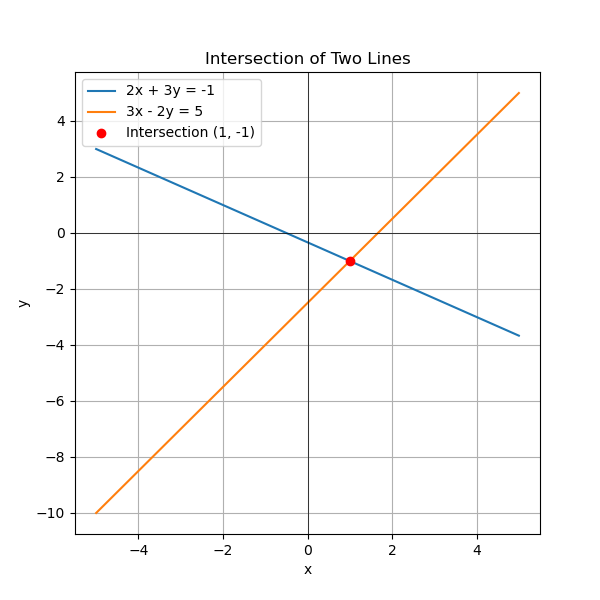
\includegraphics[width=0.7\columnwidth]{figs/fig1.png}
     \caption*{}
     \label{fig:fig1}
 \end{figure}
 
\end{frame}

\end{document}
